\documentclass{Report}
\usepackage{framed}


%% Don't import the header multiple times

\ifdefined\HEADERIMPORTED
\else
\newcommand\HEADERIMPORTED[0]{This file is HEADERIMPORTED}
\usepackage{amssymb}

\usepackage{amsmath}


% For typesetting tree rules
\usepackage{mathpartir}

% For colouring code
\usepackage{xcolor}


\usepackage{array}   % for \newcolumntype macro
\usepackage{tikz-cd}
\usepackage{tabstackengine}
\usepackage{breqn}
\usepackage{stmaryrd}

\usepackage{float} % extra options for figure placement

% For drawing boxed
\usepackage{framed}

% for code fragments + highlighting
\usepackage{listings}

% For roman numerals
\usepackage{enumitem}


\usepackage{amsthm}
%Theorems
\usepackage[utf8]{inputenc}
\usepackage[english]{babel}

\ifdefined\PRESENTATIONMODE
\else
\usepackage[a4paper,includeheadfoot,margin=2.54cm]{geometry}
\newtheorem{theorem}{Theorem}[section]
\newtheorem{corollary}{Corollary}[theorem]
\newtheorem{lemma}[theorem]{Lemma}
\newtheorem{definition}{Definition}[section]

\newtheorem{aside}{Aside}[section]
\newtheorem{property}[theorem]{Property}
\theoremstyle{definition}
\fi



\usepackage{tikz}

\definecolor{grey}{rgb}{0.75, 0.75, 0.75}
\definecolor{DarkGreen}{rgb}{0.1, 0.6, 0.1}

\usetikzlibrary{shapes.geometric,fit}
\usetikzlibrary{arrows,automata,positioning}
\usetikzlibrary{decorations.pathreplacing,calc}



\setstackEOL{\cr}
\setstackgap{L}{\normalbaselineskip}

\newcommand\todo[1]{\textbf{TODO: #1}}
\newcommand\needsRef[1]{\textbf{Reference Needed: (#1)}}
\newcommand\fixLayout[1]{\textbf{Fix Layout: #1}}


%% Rule Names
% Prefixes
\newcommand{\tprefix}[0]{T-}
\newcommand{\eprefix}[0]{E-}
\newcommand{\sprefix}[0]{S-}
\newcommand\equationalprefix[0]{Eq-}
\newcommand\envprefix[0]{Env-}
\newcommand\pprefix[0]{\eprefix\envprefix}

\newcommand\subprefix[0]{Sb-}
\newcommand\weakenprefix[0]{Wk-}

% Base  rule names
\newcommand\basenil[0]{Nil}
\newcommand\baseextend[0]{Extend}

\newcommand{\baseground}[0]{Ground}
\newcommand{\baseweaken}[0]{Weaken}
\newcommand{\basevar}[0]{Var}
\newcommand\basefn[0]{Fn}
\newcommand\baseeffect[0]{Effect}
\newcommand\basequant[0]{Quantification}


\newcommand\baseunit[0]{Unit}
\newcommand\basetrue[0]{True}
\newcommand\basefalse[0]{False}
\newcommand\baseconst[0]{Const}
\newcommand\basesubtype[0]{Subtype}
\newcommand\basegen[0]{Effect-Gen}
\newcommand\basespec[0]{Effect-Spec}
\newcommand\basereturn[0]{Return}
\newcommand\baseapply[0]{Apply}
\newcommand\baseif[0]{If}
\newcommand\basebind[0]{Bind}

\newcommand\basetransitive[0]{Transitive}
\newcommand\basereflexive[0]{Reflexive}

\newcommand{\baseid}[0]{Id}
\newcommand\baseproject[0]{Project}

% Effect Weakening Rule Names
\newcommand{\eid}[0]{\eprefix\baseid}
\newcommand{\eproject}[0]{\eprefix\baseproject}
\newcommand{\eextend}[0]{\eprefix\baseextend}

% Term Weakening Rule Names
\newcommand{\tid}[0]{\tprefix\baseid}
\newcommand{\tproject}[0]{\tprefix\baseproject}
\newcommand{\textend}[0]{\tprefix\baseextend}

% Effect Substitution Rule Names
\newcommand\esubnil[0]{\eprefix\basenil}
\newcommand\esubextend[0]{\eprefix\baseextend}

% Term Substitution Rule Names

\newcommand\tsubnil[0]{\tprefix\basenil}
\newcommand\tsubextend[0]{\tprefix\baseextend}

% Type environment Rule Names
\newcommand\envnil[0]{\envprefix\basenil}
\newcommand\envextend[0]{\envprefix\baseextend}
% Effect Environment rule names
\newcommand\pnil[0]{\pprefix\basenil}
\newcommand\pextend[0]{\pprefix\baseextend}
% Equational equality rule names
\newcommand{\eqbeta}[0]{\equationalprefix Lambda-Beta}
\newcommand{\eqeta}[0]{\equationalprefix Lambda-Eta}
\newcommand{\eqeffbeta}[0]{\equationalprefix Effect-Beta}
\newcommand{\eqeffeta}[0]{\equationalprefix Effect-Eta}
\newcommand\eqleftunit[0]{\equationalprefix Left-Unit}
\newcommand\eqrightunit[0]{\equationalprefix Right-Unit}
\newcommand\equnitequiv[0]{\equationalprefix Unit}
\newcommand\eqiftrue[0]{\equationalprefix If-True}
\newcommand\eqiffalse[0]{\equationalprefix If-False}
\newcommand\eqifeta[0]{\equationalprefix If-Eta}
\newcommand\eqassociativity[0]{\equationalprefix Associativity}

\newcommand{\eqreflexive}[0]{\equationalprefix\basereflexive}
\newcommand\eqtransitive[0]{\equationalprefix\basetransitive}
\newcommand\eqsymmetric[0]{\equationalprefix Symmetric}

\newcommand\equnit[0]{\equationalprefix\baseunit}
\newcommand\eqtrue[0]{\equationalprefix\basetrue}
\newcommand\eqfalse[0]{\equationalprefix\basefalse}
\newcommand\eqconst[0]{\equationalprefix\baseconst}
\newcommand{\eqvar}[0]{\equationalprefix\basevar}
\newcommand\eqweaken[0]{\equationalprefix\baseweaken}
\newcommand\eqfun[0]{\equationalprefix\basefn}
\newcommand\eqsubtype[0]{\equationalprefix\basesubtype}
\newcommand\eqgen[0]{\equationalprefix\basegen}
\newcommand\eqspec[0]{\equationalprefix\basespec}
\newcommand\eqreturn[0]{\equationalprefix\basereturn}
\newcommand\eqapply[0]{\equationalprefix\baseapply}
\newcommand\eqif[0]{\equationalprefix\baseif}
\newcommand\eqbind[0]{\equationalprefix\basebind}

% Term rule names
\newcommand\vunit[0]{\baseunit}
\newcommand\vtrue[0]{\basetrue}
\newcommand\vfalse[0]{\basefalse}
\newcommand\vconst[0]{\baseconst}
\newcommand{\vvar}[0]{\basevar}
\newcommand\vweaken[0]{\baseweaken}
\newcommand\vfun[0]{\basefn}
\newcommand\vsubtype[0]{\basesubtype}
\newcommand\vgen[0]{\basegen}
\newcommand\vspec[0]{\basespec}
\newcommand\vreturn[0]{\basereturn}
\newcommand\vapply[0]{\baseapply}
\newcommand\vif[0]{\baseif}
\newcommand\vbind[0]{\basebind}

%Effect rule names
\newcommand\eground[0]{\eprefix\baseground}
\newcommand\evar[0]{\eprefix\basevar}
\newcommand\eweaken[0]{\eprefix\baseweaken}
\newcommand\ecompose[0]{\eprefix Compose}

% Type rule names
\newcommand{\tground}[0]{\tprefix\baseground}
\newcommand{\tfun}[0]{\tprefix\basefn}
\newcommand{\teffect}[0]{\tprefix\baseeffect}
\newcommand{\tquant}[0]{\tprefix\basequant}

% Subtyping rule names
\newcommand{\stransitive}[0]{\sprefix\basetransitive}
\newcommand{\sreflexive}[0]{\sprefix\basereflexive}
\newcommand{\sground}[0]{\sprefix\baseground}
\newcommand{\sfun}[0]{\sprefix\basefn}
\newcommand{\seffect}[0]{\sprefix\baseeffect}
\newcommand{\squant}[0]{\sprefix\basequant}


\newcommand{\s}{\;}
\newcommand{\doin}[3]{\texttt{do}\s #1 \leftarrow #2 \s\texttt{in}\s #3\s}
\newcommand\apply[2]{#1\s#2}
\newcommand{\pifthenelse}[4]{\texttt{if}_{\textcolor{purple}{#1}}\s#2\s \texttt{then}\s #3 \s\texttt{else} \s#4\s}
\newcommand\ifthenelse[5]{\pifthenelse{#1, #2}{#3}{#4}{#5}}
\newcommand\const[1]{\texttt{k}^{\color{purple} #1}}
\newcommand\return[1]{\texttt{return} \s#1\s}


\newcommand\lam[3]{\lambda #1 \colon {\color{purple}#2}. #3\s}
\renewcommand\u[0]{\texttt{()}}
\newcommand{\U}[0]{\texttt{Unit}}
\renewcommand\t[0]{\texttt{true}}
\newcommand\f[0]{\texttt{false}}
\newcommand{\B}[0]{\texttt{Bool}}
\newcommand{\G}[0]{\Gamma}
\newcommand\D{\Delta}


% draw type relations
\newcommand{\typerelation}[3]{{\color{DarkGreen}#1} \vdash #2 \colon {\color{blue}#3}}
\newcommand\wellformed[2]{{\color{DarkGreen}#1}\vdash {\color{blue}#2}}
\newcommand\wellformedok[2]{\ok{{\color{DarkGreen}#1}\vdash {\color{blue} #2}}}

\newcommand{\wellformedtype}[2]{\typerelation{#1}{#2}{\type}}
\newcommand{\wellformedeffect}[2]{\typerelation{#1}{#2}{\effect}}
\newcommand{\wellformedF}[2]{\typerelation{#1}{#2}{F}}



\newcommand{\gtyperelation}[2]{\typerelation{\G}{#1}{#2}}
 

\newcommand\treerulez[1]{\inferrule{ }{#1}}
\newcommand\treeruleI[2]{\inferrule{#1}{#2}}
\newcommand\treeruleII[3]{\inferrule{#1 \\ #2}{#3}}
\newcommand\treeruleIII[4]{\inferrule{#1 \\ #2 \\ #3}{#4}}
\newcommand\treeruleIV[5]{\inferrule{#1 \\ #2 \\ #3 \\ #4}{#5}}
\newcommand\treeruleV[6]{\inferrule{#1 \\ #2 \\ #3 \\ #4 \\ #5}{#6}}

\newcommand\ntreerulez[2]{(\text{#1})\inferrule{ }{#2}}
\newcommand\ntreeruleI[3]{(\text{#1})\inferrule{#2}{#3}}
\newcommand\ntreeruleII[4]{(\text{#1})\inferrule{#2 \\ #3}{#4}}
\newcommand\ntreeruleIII[5]{(\text{#1})\inferrule{#2 \\ #3 \\ #4}{#5}}
\newcommand\ntreeruleIV[6]{(\text{#1})\inferrule{#2 \\ #3 \\ #4 \\ #5}{#6}}
\newcommand\ntreeruleV[7]{(\text{#1})\inferrule{#2 \\ #3 \\ #4 \\ #5 \\ #6}{#7}}

\newcommand\condtreerulez[3]{(\text{#1})\inferrule{ }{#2}(\text{if } #3)}
\newcommand\condtreeruleI[4]{(\text{#1})\inferrule{#2}{#3}(\text{if } #4)}
\newcommand\condtreeruleII[5]{(\text{#1})\inferrule{#2 \\ #3}{#4}(\text{if } #5)}
\newcommand\condtreeruleIII[6]{(\text{#1})\inferrule{#2 \\ #3 \\ #4}{#5}(\text{if } #6)}
\newcommand\condtreeruleIV[7]{(\text{#1})\inferrule{#2 \\ #3 \\ #4 \\ #5}{#6}(\text{if } #7)}
\newcommand\condtreeruleV[8]{(\text{#1})\inferrule{ #2 \\ #3 \\ #4 \\ #5 \\ #6 }{#7}(\text{if } #8)}



\newcommand{\subtype}[0]{\leq\colon}
\newcommand\subeffect[0]{\leq}

\newcommand{\M}[2]{\texttt{M}_{#1}{#2}}

\newcommand\lamtype[3]{#1 \rightarrow \M{#2}{#3}}
\newcommand{\1}[0]{\texttt{1}}

\newcommand\e[0]{\epsilon}

\newcommand{\db}[1]{{\bf [\![}#1{\bf ]\!]}}
\newcommand{\deno}[1]{\db{#1}}
\newcommand\after\circ
\newcommand\term[1]{\langle\rangle_{#1}}

\newcommand\bindmu[0]{\mu}
\newcommand\point[1]{\eta_{#1}}
\newcommand\bind[3]{\bindmu_{#1, #2, #3}}

\newcommand\T[2]{T_{#1}{#2}}

\newcommand\pr[2]{\langle#1, #2\rangle}
\newcommand\finpr[2]{\langle #1\rangle_{#2}}

\newcommand\strengtht[0]{\texttt{t}}
% tensor strength Nat-tran
\newcommand\tstrength[3]{\strengtht_{#1, #2, #3}}

% Id morphism
\newcommand\Id[1]{\texttt{Id}_{#1}}

\newcommand\idg[0]{\Id{\G}}
% beta-eta equivalence
\newcommand\beequiv[0]{\approx}
% Substitutions
\newcommand\si{\sigma}

\newcommand{\sub}[1]{[#1]}
\newcommand{\ssub}[2]{[#2 / #1]}
\newcommand{\ssi}[0]{\sub{\si}}

% beta-eta equivalence relation
\newcommand{\berelation}[4]{\typerelation{#1}{#2 \beequiv #3}{#4}}
\newcommand{\gberelation}[3]{\gtyperelation{#1 \beequiv #2}{#3}}


% Shortcuts for denotational equality
\newcommand{\denoequality}[4]{\deno{\typerelation{#1}{#2}{#4}} = \deno{\typerelation{#1}{#3}{#4}}}
\newcommand{\gdenoequality}[3]{\denoequality{\G}{#1}{#2}{#3}}

% Shorthand for monad types
\newcommand\mea[0]{\M{\e}{A}}
\newcommand\meb[0]{\M{\e}{B}}
\newcommand\mec[0]{\M{\e}{C}}

\newcommand\tea[0]{\T{\e}{A}}
\newcommand\teb[0]{\T{\e}{B}}
\newcommand\tec[0]{\T{\e}{C}}


\newcommand\moa[0]{\M{\1}{A}}
\newcommand\mob[0]{\M{\1}{B}}
\newcommand\moc[0]{\M{\1}{C}}

\newcommand\toa[0]{\T{\1}{A}}
\newcommand\tob[0]{\T{\1}{B}}
\newcommand\toc[0]{\T{\1}{C}}

\newcommand\aeb[0]{\lamtype{A}{\e}{B}}

% Shorthand for Gammas
\newcommand{\gax}[0]{\G, x\colon A}
\newcommand{\gby}[0]{\G, y\colon B}

% reduction function
\newcommand{\reduce}[0]{reduce}



% Combinators for building delta-based tree proof terms
\newcommand{\deltavrule}[4]{
    \ntreeruleII{\vsubtype}{\treeruleI{\D}{\typerelation{#1}{#2}{#3}}}{#3 \subtype #4}{\typerelation{#1}{#2}{#4}}}

\newcommand{\deltavruleprime}[4]{
    \ntreeruleII{\vsubtype}{\treeruleI{\D'}{\typerelation{#1}{#2}{#3}}}{#3 \subtype #4}{\typerelation{#1}{#2}{#4}}}

\newcommand{\deltavruleprimeprime}[4]{
        \ntreeruleII{\vsubtype}{\treeruleI{\D'}{\typerelation{#1}{#2}{#3}}}{#3 \subtype #4}{\typerelation{#1}{#2}{#4}}}
    
\newcommand{\deltacrule}[6]{
            \ntreeruleII{Subeffect}{\treeruleI{\D}{\typerelation{#1}{#2}{\M{#3}{#4}}}}{\subeffecttree{#3}{#4}{#5}{#6}}{\typerelation{#1}{#2}{\M{#5}{#6}}}}
\newcommand{\deltacruleprime}[6]{
    \ntreeruleII{Subeffect}{\treeruleI{\D'}{\typerelation{#1}{#2}{\M{#3}{#4}}}}{
    \subeffecttree{#3}{#4}{#5}{#6}}{\typerelation{#1}{#2}{\M{#5}{#6}}}}
\newcommand{\deltacruleprimeprime}[6]{
    \ntreeruleII{\vsubtype}{\treeruleI{\D''}{\typerelation{#1}{#2}{\M{#3}{#4}}}}{
        \subeffecttree{#3}{#4}{#5}{#6}}{\typerelation{#1}{#2}{\M{#5}{#6}}}}
                            

\newcommand{\p}[0]{\pi_1}
\newcommand{\pp}[0]{\pi_2}

% short-hands for weakening
\newcommand{\wrel}[3]{#1 \colon {\color{blue}#2} \triangleright {\color {blue} #3}}
\newcommand{\ok}[1]{{\color{blue} #1} \texttt{ Ok}}
\newcommand\okt[0]{\texttt{Ok}}
\renewcommand\i[0]{\iota}
\newcommand\w{\omega}
\newcommand\dom[1]{\texttt{dom}(#1)}
\newcommand\x{\times}


\newcommand\fev[1]{fev(#1)}
\newcommand\union[0]{\cup}


% Combinators to build tree proofs
\newcommand{\truleconst}[0]{\ntreeruleI{\vconst}{\ok{\G}}{\gtyperelation{\const{A}}{A}}}
\newcommand{\truleunit}[0]{\ntreeruleI{\vunit}{\ok{\G}}{\typerelation{\G}{\u}{\U}}}
\newcommand{\truletrue}[0]{\ntreeruleI{\vtrue}{\ok{\G}}{\typerelation{\G}{\t}{\B}}}
\newcommand{\trulefalse}[0]{\ntreeruleI{\vfalse}{\ok{\G}}{\typerelation{\G}{\f}{\B}}}


\newcommand{\E}[0]{\mathbb{E}}
\renewcommand{\dot}{\cdot}
\newcommand{\gens}[0]{\colon\colon=}
\newcommand{\nil}[0]{\diamond}
\newcommand{\ground}[0]{\gamma}

% Terminal object of C
\newcommand{\terminal}[0]{\texttt{\1}}

% The category C
\newcommand{\C}[0]{\mathbb{C}}
\newcommand{\Cz}[0]{\C_0}
\newcommand\DC[0]{\mathbb{D}}

% The category of locally-small categories
\newcommand{\Cat}[0]{\texttt{Cat}}
% Sub-effect Nat-trans
\newcommand{\dse}[2]{\db{#1 \subeffect #2}}

\newcommand\app[0]{\texttt{app}}
\newcommand\cur[1]{\texttt{cur}(#1)}
\newcommand{\ifnt}[1]{\texttt{If}_{#1}}


\newcommand{\setto}{\colon=}
\newcommand{\fv}[1]{\texttt{fv}(#1)}

% shorthand for inserting text to equations
\newcommand\qt[1]{\quad\text{#1}}

% Co-product short-hands
\newcommand\inr[0]{\texttt{inr}}
\newcommand\inl[0]{\texttt{inl}}
    
\newcommand\fld[2]{[#1,#2]}
\newcommand{\diag}[1]{\delta_{#1}}
\newcommand{\twist}[2]{\tau_{#1, #2}}

\newcommand\ifMorph[3]{\app\after((\fld{\cur{#2\after\pp}}{\cur{#3\after\pp}}\after #1)\times \idg)\after \diag{\G}}


% Polymorphic short-hands
\newcommand\elam[2]{\Lambda #1. #2}
\newcommand{\eapp}[2]{#1\s#2}
\renewcommand{\a}[0]{\alpha}
\newcommand{\all}[2]{\forall #1. #2}
\renewcommand{\P}[0]{\Phi}

\renewcommand{\b}[0]{\beta}
\newcommand{\g}[0]{\gamma}
\renewcommand\d[0]{\delta}
\newcommand\oke[2]{\wellformedok{#1}{#2}}
\newcommand\etyperelation[4]{\typerelation{#1\mid#2}{#3}{#4}}
\newcommand{\gpetyperelation}[2]{\etyperelation{\P}{\G}{#1}{#2}}
\newcommand{\gppetyperelation}[2]{\etyperelation{\P'}{\G}{#1}{#2}}


\newcommand{\eberelation}[5]{\berelation{#1\mid#2}{#3}{#4}{#5}}
\newcommand{\gpeberelation}[3]{\berelation{\P\mid\G}{#1}{#2}{#3}}
\newcommand{\gppeberelation}[3]{\berelation{\P'\mid\G}{#1}{#2}{#3}}

\newcommand{\dotp}[0]{\dot_\P}
\newcommand{\fntype}[2]{#1\rightarrow #2}
\newcommand{\ab}[0]{\fntype{A}{B}}

\newcommand\wrelw[2]{\wrel{\w}{#1}{#2}}
\renewcommand\proof[0]{\paragraph{Proof:}}
\newcommand{\case}[1]{\paragraph{Case #1:}}
\newcommand{\subcase}[1]{\subparagraph{Case: #1}}
\newcommand\bi[0]{By inversion}

%pre-filled effect-weakening relations
\newcommand\ewrel[4]{\wellformed{#1}{\color{black}\wrel{#2}{#3}{#4}}}
\newcommand\pewrel[3]{\ewrel{\P}{#1}{#2}#3}
\newcommand\ppewrel[3]{\ewrel{\P'}{#1}{#2}#3}

\newcommand\subtypep[0]{\subtype_\P}
\newcommand\subtypepp[0]{\subtype_{\P'}}
\newcommand\subeffectp[0]{\subeffect_{\P}}
\newcommand\subeffectpp[0]{\subeffect_{\P'}}
\newcommand\subeffectn[0]{\subeffect_{n}}
\newcommand\subeffectz[0]{\subeffect_{0}}

\newcommand{\allI}[0]{\forall_I}
\newcommand{\allII}[0]{\forall_{I'}}
\newcommand\allIU[0]{\forall_{I\times U}}
\newcommand\type[0]{\texttt{Type}}
\newcommand\effect[0]{\texttt{Effect}}
\newcommand\ciw[0]{\C(I, W)}
\newcommand\ciu[0]{\C(I, U)}
\newcommand\ciuw[0]{\C(I\times U, W)}
\newcommand\cipw[0]{\C(I', W)}
\newcommand\cipu[0]{\C(I', U)}
\newcommand\ciuu[0]{\C(I\times U, U)}
\newcommand\cii[0]{\C(I', I)}
\newcommand\Eff[0]{\texttt{Eff}}
\newcommand\Mul[0]{\texttt{Mul}}
\newcommand\singleton[0]{\ast}
\renewcommand\star[0]{^*}
\renewcommand\bar[1]{\overline{#1}}

\newcommand\subtypeg[0]{\subtype_\g}
\newcommand\subtypepa[0]{\subtype_{\P, \a}}
\newcommand\subtypeppa[0]{\subtype_{\P', \a}}

\newcommand\subtypez[0]{\subtype_{0}}
\newcommand\subtypen[0]{\subtype_{n}}

\usepackage{scalerel,stackengine}
\stackMath
\renewcommand\widehat[1]{%
\savestack{\tmpbox}{\stretchto{%
  \scaleto{%
    \scalerel*[\widthof{\ensuremath{#1}}]{\kern.1pt\mathchar"0362\kern.1pt}%
    {\rule{0ex}{\textheight}}%WIDTH-LIMITED CIRCUMFLEX
  }{\textheight}% 
}{2.4ex}}%
\stackon[-6.9pt]{#1}{\tmpbox}%
}
\parskip 1ex

\newcommand\pstar[0]{\p\star}

\newcommand\edeltavrule[5]{\deltavrule{#1 \mid #2}{#3}{#4}{#5}}

\newcommand\subeffecttreep[4]{\ntreeruleII{\teffect}{
    #1\subeffectp #3}{#2 \subtypep #4
}{\M{#1}{
    #2
}\subtypep\M{#3}{#4}}}
\newcommand\subeffecttree[4]{\ntreeruleII{\teffect}{
    #1\subeffect #3}{#2 \subtype #4
}{\M{#1}{
    #2
}\subtype\M{#3}{#4}}}


\newcommand{\edeltavruleprime}[5]{
        \deltavruleprime{#1\mid #2}{#3}{#4}{#5}}
    
\newcommand{\edeltavruleprimeprime}[5]{
        \deltavruleprimeprime{#1\mid #2}{#3}{#4}{#5}}
    
\newcommand{\edeltacrule}[6]{
            \ntreeruleII{\vsubtype}{
                \treeruleI{
                    \D
                }{
                    \typerelation{\P\mid#1}{#2}{\M{#3}{#4}}
                }
            }{
                \ntreeruleII{\teffect}{
                    #4 \subtypep #6
                    }{
                         #3 \subeffectp #5
                }{
                    \M{#3}{#4}\subtypep{\M{#5}{#6}}
                }
            }{
                \typerelation{\P\mid #1}{#2}{\M{#5}{#6}}
            }
        }
        

        \newcommand{\edeltacruleprime}[6]{
            \ntreeruleII{\vsubtype}{
                \treeruleI{
                    \D'
                }{
                    \typerelation{\P\mid #1}{#2}{\M{#3}{#4}}
                }
            }{
                \ntreeruleII{\teffect}{
                    #4 \subtypep #6
                }{#3 \subeffectp #5
                }{
                    \M{#3}{#4}\subtypep{\M{#5}{#6}}
                }
            }{
                \typerelation{\P\mid #1}{#2}{\M{#5}{#6}}
            }
        }
                   

        \newcommand{\edeltacruleprimeprime}[6]{
            \ntreeruleII{\vsubtype}{
                \treeruleI{
                    \D''
                }{
                    \typerelation{\P\mid #1}{#2}{\M{#3}{#4}}
                }
            }{
                \ntreeruleII{\teffect}{
                    #4 \subtypep #6
                    }{ #3 \subeffectp #5
                }{
                    \M{#3}{#4}\subtypep{\M{#5}{#6}}
                }
            }{
                \typerelation{\P\mid #1}{#2}{\M{#5}{#6}}
            }
        }

        \newcommand\obj[0]{\texttt{obj }}


        \newcommand{\Tz}[2]{\texttt{T}^0_{#1}#2}
        \newcommand{\Tn}[2]{\texttt{T}^n_{#1}#2}
        \newcommand{\Tm}[2]{\texttt{T}^m_{#1}#2}
        
        \newcommand{\pointz}[1]{\point{#1}^0}
        \newcommand{\pointn}[1]{\point{#1}^n}
        \newcommand{\pointm}[1]{\point{#1}^m}
        
        \newcommand{\bindz}[3]{\bind{#1}{#2}{#3}^0}
        \newcommand{\bindn}[3]{\bind{#1}{#2}{#3}^n}
        \newcommand{\bindm}[3]{\bind{#1}{#2}{#3}^m}
        
        \newcommand\tstrengthz[3]{\tstrength{#1}{#2}{#3}^0}
        \newcommand\tstrengthn[3]{\tstrength{#1}{#2}{#3}^n}
        \newcommand\tstrengthm[3]{\tstrength{#1}{#2}{#3}^m}
        
        \newcommand\set[0]{\texttt{Set}}
        \newcommand\cccat[0]{\textit{CCCat}}

        \newcommand\ev[0]{\vec{\e}}
        \newcommand\emv[0]{\vec{\e_m}}
        \newcommand\env[0]{\vec{\e_n}}
        
        \newcommand\subeffectm[0]{\subeffect_m}
        
        \newcommand\dsem[2]{\db{#1 \subeffectm #2}}
        \newcommand\dsen[2]{\db{#1 \subeffectn #2}}
        \newcommand\dsez[2]{\db{#1 \subeffectz #2}}
        \newcommand\dsep[2]{\db{#1 \subeffectp #2}}
        \newcommand\dsepp[2]{\db{#1 \subeffectpp #2}}
        
        \newcommand\allEn[0]{\forall_{E^n}}
        \newcommand\allEm[0]{\forall_{E^m}}
        
        \newcommand\counit[1]{\boldsymbol{\epsilon}_{#1}}
        \newcommand\unit[1]{\boldsymbol{\eta}_{#1}}


        
%% Adequacy shorthands
\newcommand{\relates}[0]{\lhd}
\newcommand{\logRel}[3]{#1 \relates_{#2} #3}
\newcommand{\plogRel}[4]{#1 \relates_{\wellformed{#2}{#3}} #4}

\newcommand{\zberelation}[3]{\berelation{}{#1}{#2}{#3}}
\newcommand\ztyperelation[2]{\typerelation{}{#1}{#2}}

\newcommand{\N}[0]{\mathbb{N}}
\renewcommand\put[0]{\texttt{put}}
\newcommand\ecput[0]{\texttt{EC}_\put}
\newcommand\ecputA[0]{\texttt{EC}_\put^A}
\newcommand\ecputG[0]{\texttt{EC}_\put^G}

\newcommand\mna[0]{\M{n}{A}}
\newcommand\mmb[0]{\M{m}{B}}
\newcommand\mnb[0]{\M{n}{B}}
\newcommand\mma[0]{\M{m}{A}}

\newcommand{\setcomp}[2]{\{#1 \mid #2 \}}
\fi

\usepackage{tikz}

\usetikzlibrary{shapes.geometric,fit}
\usetikzlibrary{arrows,automata,positioning}
\usetikzlibrary{decorations.pathreplacing,calc}


\begin{document}
\abstract


    
To date, there has been limited work on the semantics of languages with polymorphic effect systems. The application, by Moggi, of strong monads to modelling the semantics of effects has become a mainstream concept in functional programming languages. This was improved upon by Lucasson (?) using a graded monad to model languages with a range of independent and dependent effects at an operational level. A categorical semantics for parametric polymorphism in types was first published by Reynolds (?) allowing a denotational analysis of languages including type parameters. There has been some work on polymorphism over the exception effect (which paper). Despite these works, there has been no work to date on the denotational semantics of languages with general parametric polymorphism over effects.

In this dissertation, I present several pieces of work. Firstly, I shall introduce a modern definition of a lambda-calculus based language with an explicit graded monad to handle a variety of effects. This calculus shall then be extended using polymorphic terms to yield a more general polymorphic-effect-calculus. I shall then give an indexed-category-based denotational semantics for the language, along with an outline of a proof for the soundness of these semantics. Following this, I shall present a method of transforming a model of a non-polymorphic language into a model of the language with polymorphism over effects.

The full proofs can be found online on my github repository (link), since due to the number of theorems and cases, the total size is well over 100 pages of definitions, theorems, and proofs.

\chapter{Introduction}
\section{What is Effect Polymorphism?}
Effect polymorphism is when the same function in a language can operate on values of similar types but with different effects. It allows the same piece of code to be used in multiple contexts with different type signatures. This manifests in a similar manner to type parameter polymorphism in system-F based languages. Consider the following Scala-style pseudo-code:

\begin{framed}
    \begin{framed}
        \begin{verbatim}
def check[E: Effect](
    action: Unit => (Unit;e)
): Unit; (IO, e) {
    val ok: Boolean = promptBool(
        "Are you sure you want to do this?"
    )
    If (ok) {
        action()
    } else {
       abort()
    }
}  
            \end{verbatim}
    \end{framed}

    \begin{framed}
        \begin{verbatim}
check[RealWorld](() => check[RealWorld](FireMissiles))
check[Transaction](SendMoney(Bob, 100, USD))
check[Exception](ThrowException("Not Aborted"))
        \end{verbatim}
    \end{framed}
\end{framed}

In this example, we are reusing the same “check” function in three different cases with three different effects in a type safe manner. Hence, “check” is polymorphic in the effect parameter it receives. To analyse this language, it would be useful to have an analysis tool that can precisely model these separate, though potentially interdependent effects. A denotational semantics that can account for the parametric polymorphism over effects would be a step towards building such tools.

\section{An Introduction to Categorical Semantics}
In this dissertation, I shall be describing a denotational semantics using category theory. A denotational semantics for a language is a mapping, known as a denotation, $\deno{-}$, of structures in the language, such as types and terms to mathematical objects in such a way that non-trivial properties of the terms in the language correspond to other properties of the denotations of the terms.

When we specify a denotational semantics of a language in category theory, we look to find a mapping of types and typing environments to objects in a given category.

\begin{align}
    A: \type & \mapsto \deno{A} \in \obj \C \\
    \G & \mapsto  \deno{\G} \in \obj \C
\end{align}



Further more, instances of the type relation should be mapped to morphisms between the relevant objects.

\begin{align}
    \gtyperelation{v}{A} & \mapsto \C(\deno{\G}, \deno{A}) 
\end{align}

This should occur in a sound manner. That is, for every instance of the $\beta\eta$-equivalence relation between two terms, the denotations of the terms should be equal in the category.

\begin{align}
    \gberelation{v_1}{v_2}{A} & \implies \deno{\gtyperelation{v_1}{A}} = \deno{\gtyperelation{v_2}{A}}
\end{align}

An example of $\beta\eta$-equivalence is that of the $\beta$-reduction of lambda terms. It should be the case that:

\begin{align}
    \treerule{Lambda-Beta}{\typerelation{\gax}{v_1}{B}\s\s\gtyperelation{v_2}{A}}{\gberelation{\apply{(\lam{x}{A}{v_1})}{v_2}}{v_1\ssub{x}{v_2}}{B}}
\end{align}

Means that the denotations $\deno{\gtyperelation{\apply{(\lam{x}{A}{v_1})}{v_2}}{B}}$ and $\deno{\gtyperelation{v_1\ssub{x}{v_2}}{B}}$ are equal.

To prove soundness, we perform rule induction over the derivation of the $\beta\eta$-equivalence relation, such as the lambda-beta-reduction rule above. 

Some of the inductive cases require us to quantify what the substitution of terms for variables, such as $\ssub{x}{v_1}$ does to the denotations of the parent term. Substitution theorems, allow us to quantify this action on denotations in a category theoretic way. 

If \begin{equation}
    \typerelation{\gax}{v_1}{B}
\end{equation}

And \begin{equation}
    \typerelation{\G}{v_2}{A}
\end{equation}

Then \begin{equation}
    \deno{\typerelation{\G}{v_1\ssub{x}{v_2}}{B}}
\end{equation}

Should be derivable from

\begin{equation}
    \deno{\typerelation{\gax}{v_1}{B}}
\end{equation}

And  \begin{equation}
    \deno{\gtyperelation{v_2}{A}}
\end{equation}

A similar concept is that of environment weakening. $\gax$ can derive every typing relation that $\G$ can, if $x$ is not already in the environment $\G$. Hence, $\gax$ is an example of a typing environment that is \textit{weaker} than $\G$. A weakening theorem proves that there is a systematic way to generate the denotation of a typing-relation on a term in a weaker environment from the denotation of the same term in a stronger environment.

If \begin{equation}
    \G' \leq_{\text{weaker}} \G
\end{equation}

Then

\begin{equation}
    \deno{\typerelation{\G'}{v}{A}}
\end{equation}

should be derivable from

\begin{equation}
    \deno{\typerelation{\G}{v}{A}}
\end{equation}

\subsection{Languages and Their Requirements}
Different languages require different structures to be present in a category for the category to be able to interpret terms in the language. Using the concepts defined in \ref{CategoryTheoryRequirements}, I shall now give an introduction to which category-theoretic structures are required to interpret different language features. 

One of the simplest, while still interesting, languages to derive a denotational semantics for is the simply typed lambda calculus (STLC). STLC's semantics require a cartesian closed category (CCC, see section \ref{CCC}).

Products in the CCC are used to denote the lists of variable types in the typing environment, exponential objects model functions, and the terminal object is used to derive representations of ground terms, such as the unit term, $()$, as well as the empty typing environment.


\begin{itemize}
    \item Products are used to construct type environments. $\deno{\G} = \deno{\nil, x: A, y:B, ... z:C} = \1 \times \deno{A} \times \deno{B} \times ... \times \deno{C}$
    \item Terminal objects are used in the denotation of constant terms $\deno{\gtyperelation{\const{A}}{A}} = \deno{\const{A}}\after\term{\deno{\G}}$
    \item Exponentials are used in the denotations of functions. $\deno{\typerelation{\G}{\lam{x}{A}{v}}{\ab}} = \cur{\deno{\typerelation{\gax}{v}{B}}}$
\end{itemize}

From this, we can specify what structures categories need to have in order to model more complex languages.
\begin{center}
    \begin{tabular}{|c|c|}
        \hline
        Language Feature & Structure Required \\
        \hline
        \hline
        STLC            & CCC \\
        \hline
        If expressions and booleans   & Co-product on the terminal object \\
        \hline
        Single Effect   & Strong Monad \\
        \hline
        Multiple Effects & Strong Graded Monad \\
        \hline
        Polymorphism & Indexed Category \\
        \hline
    \end{tabular}
\end{center}


A single effect can be modelled by adding a strong monad to the category, as shown by Moggi \todo{Reference}. The monad allows us to generate a unit effect and to compose multiple instances of the effect together in a way that intuitively matches the type system of a monadic language.

\begin{eqnarray}\label{MonadTypeRules}
    \treerule{Return}{\typerelation{\G}{v}{A}}{\typerelation{\G}{\return{v}}{\M{}{A}}} & \treerule{Bind}{\typerelation{\G}{v_1}{\M{}{A}} \s\s \typerelation{\gax}{v_2}{\M{}{B}}}{\typerelation{\G}{\doin{x}{v_1}{v_2}}{\M{}{B}}}
\end{eqnarray}

These type rules can be modelled using the ``unit'' natural transformation and a combination of the ``join'' and tensor strength natural transformations respectively. 

For a more precise analysis of languages with multiple effects, we can look into the algebra on the effects. A simple example of such an algebra is a partially ordered monoid. The monoid operation defines how to compose effects, and the partial order gives a sub-typing relation to make programming more intuitive with respect to if statements. A category with a strong graded monad allows us to model this algebra in a category theoretic way. It also allows us to do some effect analysis in the type system, as seen in the type rules for return and bind in equation \ref{GradedMonadTypeRules}.

\begin{eqnarray}\label{GradedMonadTypeRules}
    \treerule{Return}{\typerelation{\G}{v}{A}}{\typerelation{\G}{\return{v}}{\moa}} & \treerule{Bind}{\typerelation{\G}{v_1}{\M{\e_1}{A}} \s\s \typerelation{\gax}{v_2}{\M{\e_2}{B}}}{\typerelation{\G}{\doin{x}{v_1}{v_2}}{\M{\e_1 \dot \e_2}{B}}}
\end{eqnarray}


To express polymorphism over a property $P$, the language's semantics are expanded to use a new environment specifying the variables ranging over $P$ that are allowed in a given context. This can be seen in the augmented type rules in \ref{PolymorphismTypeRules}.

\begin{eqnarray}\label{PolymorphismTypeRules}
    \treerule{Gen}{\etyperelation{\P, \a}{\G}{v}{A}}{\gpetyperelation{\elam{\a}{v}}{\all{\a}{A}}}& \treerule{Spec}{\gpetyperelation{v}{\all{\a}{A}}\s\s\wellformed{\P}{\e}}{\gpetyperelation{\eapp{v}{\e}}{A\ssub{\a}{\e}}}
\end{eqnarray}

To model these augmented type rules, we can create a category representing the semantics (an S-Category) of the non-polymorphic language at each given context. This collection of non-polymorphic categories can be indexed by a base category which models the operations and relationships between the $P$-Environment. Morphisms in the base category between environments correspond to re-indexing functors between the S-categories for the relevant environments. These functors, and a right adjoint for the re-indexing functor corresponding to $\p$ morphism can then be used to construct the semantics of polymorphic terms. Figure \ref{IndexDiagram} demonstrates this construction.

In this dissertation, I shall show how these category theoretic building blocks can be put together to give the class of categories that can model polymorphic effect systems.

\begin{figure}[h!]\label{IndexDiagram}
    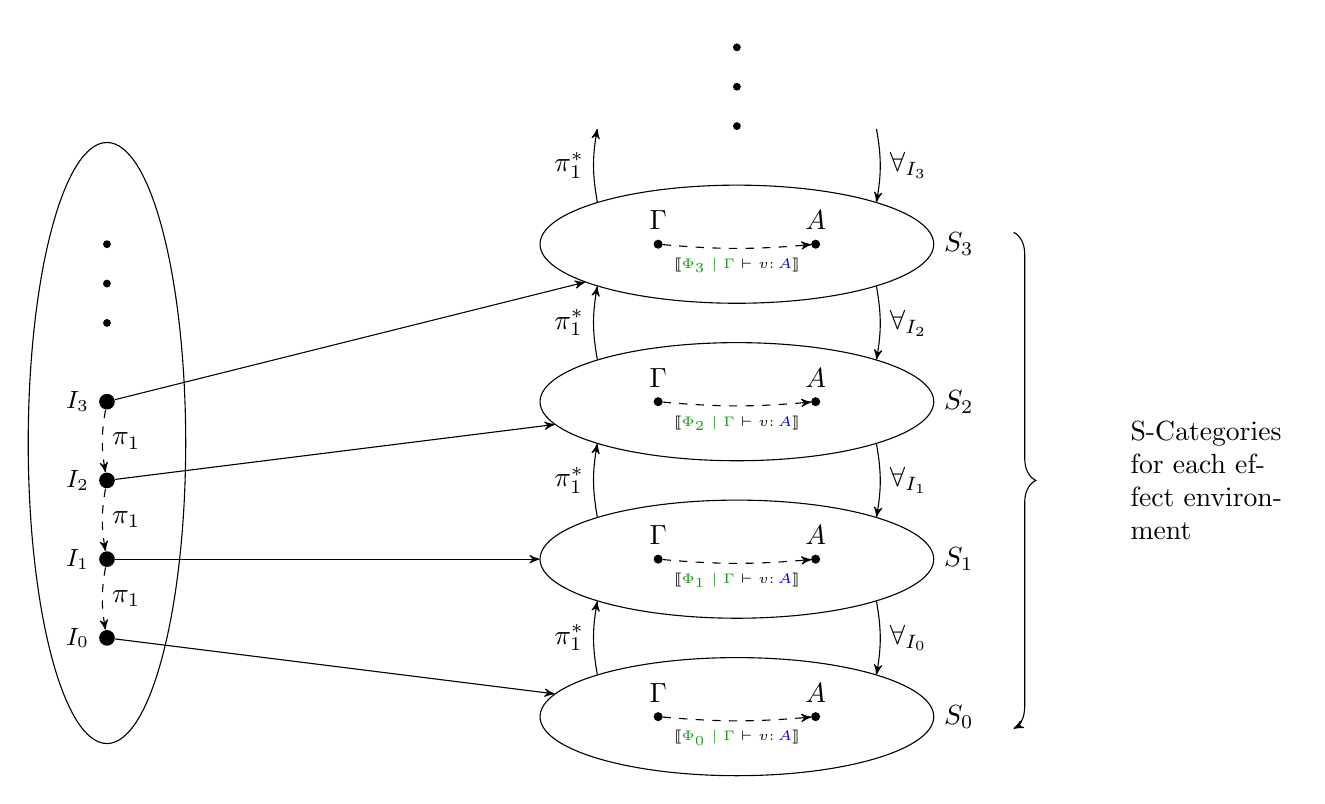
\begin{tikzpicture}[->,>=stealth']]
        % Draw the env objects
        \foreach \y[count=\c,evaluate={\yi=int(\c-1)}] in {3, 4, 5, 6}{
            \node[fill,circle,inner sep=2pt,label=left:{\small $I_\yi$}] (d\yi) at (0,\y) {};
        }

        % draw the ... above the env objects
        \foreach \y[count=\c,evaluate={\yi=int(\c-1)}] in {7, 7.5, 8}{
            \node[fill, circle, inner sep=1pt] (dd\yi) at (0,\y){};
        }
        % Draw the index category
        \node[fit=(d0) (d1) (d2) (d3) (dd0) (dd1) (dd2),ellipse,draw,minimum width=2cm] {};

        %draw the s-category stack
        \foreach \y[count=\c,evaluate={\yi=int(\c-1)}] in {2, 4, 6, 8}{
            \node[circle, draw, inner sep=1pt, fill, label=above:{$\G$}] (g\yi) at (7,\y){};
            \node[circle, draw, inner sep=1pt, fill, label=above:{$A$}] (a\yi) at (9,\y){};
            \draw[->, dashed](g\yi) to[bend right=5] node[below]{\tiny $\deno{\etyperelation{\P_\yi}{\G}{v}{A}}$} (a\yi);
            \node[ellipse, draw, minimum width=5cm, minimum height=15mm,label=right:$S_\yi$] (s\yi) at (8,\y){};
        }

        % Hidden ellipse to draw functors to
        \node[ellipse, minimum width=5cm, minimum height=15mm] (s4) at (8,10){};

        %Draw the ... for the s-category stack
        \foreach \y[count=\c,evaluate={\yi=int(\c-1)}] in {9.5, 10, 10.5}{
            \node[fill, circle, inner sep=1pt] (p\yi) at (8, \y){};
        }

        % Draw index arrows
        \foreach \i in {0, 1, 2, 3}{
            \draw[->] (d\i) to (s\i);
        }

        % draw the re-indexing functors

        \foreach \source[count=\dest] in {0, 1, 2, 3}{
            \draw[->](s\source.north west) to[bend left=10] node[left]{$\pstar$} (s\dest.south west);
        }

        % Draw the quantification functors
        \foreach \dest[count=\source] in {0, 1, 2, 3}{
            \draw[->] 
            (s\source.south east) to[bend left=10] node[right]{$\forall_{I_\dest}$} (s\dest.north east);
        }

        % Draw the internal morphisms in base category
        \foreach \dest[count=\source] in {0, 1, 2}{
            \draw[dashed,->]
            (d\source) to[bend right=10] node[right]{$\p$} (d\dest);
        }

        %Draw the bracket

        \draw [decoration={brace,amplitude=8pt},decorate] ($(s3)+(10em,1ex)$) -- ($(s0)+(10em,-1ex)$);
        \node[text width=20mm] (Label) at (14,5){S-Categories for each effect environment};
    \end{tikzpicture}
    \caption{Diagram of the structure of an indexed category for modelling a polymorphic language. Solid arrows represent functors and dashed arrows represent internal morphisms. The left hand category is the base category.}
\end{figure}

\chapter{Required Category Theory}\label{CategoryTheoryRequirements}

Before going further, it is necessary to assert a common level of category theory knowledge. This section is not intended as a tutorial but as a to jog the memory of the reader, and briefly introduce some new concepts.

\section{Cartesian Closed Category}\label{CCC}

Recall that a category is cartesian closed if it has a terminal object, products for all pairs of objects, and exponentials.

\subsection{Terminal Object}
An object, $\1$, is terminal in a category, $\C$ if for all objects $X\in\obj\C$, there exists exactly one morphism $\term{X}: X \rightarrow \1$.

\subsection{Products}
There is a product for a pair of objects $X, Y\in\obj\C$ if there exists an object and morphisms in C:
\begin{tikzcd}
    X & \arrow{l}[swap]{\p} (X\times Y) \arrow [r, "\pp"] & Y
\end{tikzcd}

Such that for any other object and morphisms,

\begin{tikzcd}
    X & \arrow{l}[swap]{f} Z \arrow [r, "g"] & Y
\end{tikzcd}

There exists a unique morphism $\pr{f}{g}: Z \rightarrow (X\times Y)$ such that the following commutes:

\begin{tikzcd}
    & \arrow{dl}[swap]{f} Z  \arrow[d, "\pr{f}{g}"] \arrow [dr, "g"] & \\
    X & \arrow [l, "\p"] (X\times Y) \arrow{r}[swap]{\pp} & Y\\
\end{tikzcd}

\subsection{Exponentials}
A category has exponentials if for all objects $A, B$, it has an object $B^A$ and a morphism $\app: \B^A \times A \rightarrow B$ and for each $f: (A\times B)\rightarrow C$ in $\C$ there exists a unique morphism $\cur{f}: A \rightarrow C^B$ such that the following diagram commutes.

\begin{tikzcd}
    C^B \times B \arrow{r}{\app}& C\\
    A\times B\arrow{u}{\cur{f}\times \Id{B}} \arrow{ur}{f}    
\end{tikzcd}

\section{Initial Object}

An initial object, $I$ of $\C$ is one such that for every other object $X\in\obj\C$, there exists a unique morphism $\i_X: I\rightarrow X$. It is the conceptual dual of a terminal objects.

\section{Co-Product}
A co-product is the conceptual dual of a product.

There is a co-product for a pair of objects $X, Y\in\obj\C$ if there exists an object and morphisms in C:
\begin{tikzcd}
    X  \arrow{r}[swap]{\inl} & (X + Y) & \arrow [l, "inr"]  Y
\end{tikzcd}

Such that for any other object and morphisms,

\begin{tikzcd}
    X \arrow{r}[swap]{f} & Z & \arrow [l, "g"]  Y
\end{tikzcd}

There exists a unique morphism $[f, g]: X + Y \rightarrow Z $ such that the following commutes:


\begin{tikzcd}
    &  Z   & \\
    X \arrow{ur}{f} \arrow [r, "\inl"] &  \arrow{u}{[f, g]} (X + Y)  & \arrow{l}[swap]{\inr} \arrow{ul}[swap]{g} Y\\
\end{tikzcd}



\section{Functors}
A functor $F: \C \rightarrow \DC$ is a mapping of objects:
\begin{align}
    A\in\obj\C \mapsto FA \in \obj\DC
\end{align}

And morphisms:

\begin{align}
    f: \C(A, B) \mapsto F(f): \DC(FA, FB)
\end{align}

that preserves the category properties of composition and identity.

\begin{align}
    F(\Id{A}) & = \Id{FA} \\
    F(g\after f) & = F(g)\after F(f)
\end{align}

\section{Natural Transformations}

A natural transformation $\theta$ between to functors $F, G: \C \rightarrow \DC$ is a collection of morphisms, indexed by objects in $\C$ with  $\theta_A: F(A) \rightarrow G(A)$ such that following diagram commutes for each $f: A \rightarrow B \in \C$

\begin{tikzcd}
    F(A) \arrow{r}{\theta_A} \arrow{d}{F(f)}  & G(A) \arrow{d}{G(f)}\\
    F(B) \arrow{r}{\theta_B}& G(B)\\ 
\end{tikzcd}

\section{Monad}

A monad is famously ``a monoid on the category of endofunctors''. In less opaque terms, a monad is:

\begin{itemize}
    \item A functor from $\C$ onto itself. (An endofunctor) $T: \C \rightarrow C$
    \item A ``unit'' natural transformation $\point{A}: A\rightarrow T(A)$
    \item A ``join'' natural transformation $\mu_{A}: T(T(A)) \rightarrow T(A)$
\end{itemize}

Such that the following diagrams commute:

\subsection{Associativity}
\begin{tikzcd}
    T(T(T(A)) \arrow{r}{\mu_{T(A)}} \arrow{d}{T(\mu_{A})} & T(T(A)) \arrow{d}{\mu_A} \\
    T(T(A)) \arrow{r}{\mu_A} & T(A)    
\end{tikzcd}


\subsection{Left and Right Unit}
\begin{tikzcd}
    T(A) \arrow{r}{\point{T(A)}} \arrow{d}{T(\point{A})} \arrow[equal]{rd} & T(T(A)) \arrow{d}{\mu_A}\\
    T(T(A)) \arrow{r}{\mu_A} & T(A)
\end{tikzcd}



\section{Graded Monad}
A graded monad is a generalisation of a monad to be indexed by a monoidal algebra $E$. It is made up of:

\begin{itemize}
    \item An endo-functor indexed by a monoid: $\T{}{}: (\E, \dot\, \1)  \rightarrow [\C, \C]$
    \item A unit natural transformation: $\point{}: \Id{} \rightarrow \T{\1}{}$
    \item A join natural transformation: $\bind{\e_1}{\e_2}{}: \T{\e_1}{\T{\e_2}{}} \rightarrow \T{\e_1 \dot \e_2}{}$
\end{itemize}

Such that the following diagrams commute.:
\subsection{Left and Right  Units}
    \begin{tikzcd}[ampersand replacement=\&]
        \tea
         \arrow[equal]{rd} 
         \arrow[r, "\T{\e}{\point{A}}"]
         \arrow{d}{\point{\tea}}
        \& 
        \T{\e}{\T{\1}{A}} 
            \arrow[d, "\bind{\e}{\1}{A}"] \\
            \T{\1}{\T{\e}{A}}
                 \arrow{r}{\bind{\1}{\e}{A}}
        \& 
        \tea
    \end{tikzcd}

\subsection{Associativity}
\begin{tikzcd}[ampersand replacement=\&]
    \T{\e_1}{\T{\e_2}{\T{\e_3}{A}}} 
    \arrow [r, "\bind{\e_1}{\e_2}{\T{\e_3}{A}}"]
    \arrow [d, "\T{\e_1}{\bind{\e_2}{\e_3}{A}}"] \& \T{\e_1 \dot \e_2}{\T{\e_3} A} \arrow [d, "\bind{\e_1 \dot \e_2}{\e_3}{A}"] \\
    \T{\e_1}{\T{\e_2 \dot \e_3}{A}} \arrow [r, "\bind{\e_1}{\e_2 \dot \e_3}{A}"] \& \T{\e_1 \dot \e_2 \dot \e_3}{A}    
\end{tikzcd}


\section{Tensor Strength}
Tensorial strength over a graded monad gives us the tools necessary to manipulate monadic operations in an intuitive way. A monad with tensor strength is referred to as ``strong''. Tensorial strength consists of a natural transformation:

\begin{align}
    \tstrength{\e}{A}{B}: A \times \teb \rightarrow \T{\e}{(A \times B)}
\end{align}

Such that the following diagrams commute:
\subsection{Left Naturality}
\begin{tikzcd}[ampersand replacement=\&]
    A \times \teb \arrow [r, "\Id{A} \times \T{\e}{f}"] \arrow [d, "\tstrength{\e}{A}{B}"]\&
    A \times \T{\e}{B'} \arrow [d, "\tstrength{\e}{A}{B'}"]\\
    \T{\e}{(A \times B)} \arrow [r, "\T{e}{(\Id{A} \times f)}"] \&
    \T{\e}{(A \times B')}
\end{tikzcd}

\subsection{Right Naturality}

\begin{tikzcd}[ampersand replacement=\&]
    A \times \teb  \arrow [r, "f \times \Id{\teb}"] \arrow [d, "\tstrength{\e}{A}{B}"]  \&
    A' \times \teb \arrow [d, "\tstrength {\e} {A'}{B}"]\\
    \T{\e}{(A \times B)} \arrow [r, "\T{\e}{(f \times \Id{B})}"]\&
    \T{\e}{(A' \times B)}
\end{tikzcd}

\subsection{Unitor Law}
\begin{tikzcd}[ampersand replacement=\&]
    \1 \times \tea 
    \arrow [r, "\tstrength{\e}{\1}{A}"]
    \arrow [rd, "\lambda_{\tea}"]
    \& 
    \T{\e}{(\1 \times A)}
    \arrow [d, "\T{\e}{(\lambda_A)}"]
    \\
    \&
    \tea
\end{tikzcd}
Where $\lambda: \terminal \times \Id{} \rightarrow \Id{}$ is the left-unitor.
($\lambda = \pp$)

\paragraph{Tensor Strength and Projection}
Due to the left-unitor law, we can develop a new law for the commutativity of $\pp$ with $\tstrength{}{}{}$

    $$\pi_{2, A, B} = \pi_{2, \1, B} \after (\term{A} \times \Id{B})$$

    And $\pi_{2, \1}$ is the left unitor, so by tensorial strength:
    
    \begin{equation}
        \begin{split}
            \T{\e}{\pp} \after \tstrength{\e}{A}{B} & = \T{\e}{\pi_{2, \1, B}} \after \T{\e}{(\term{A} \times \Id{B})} \after \tstrength{\e}{A}{B} \\
            & = \T{\e}{\pi_{2, 1, B}} \after \tstrength{\e}{\1}{B} \after (\term{A} \times \Id{B}) \\
            & = \pi_{2,1,B} \after (\term{A} \times \Id{B}) \\
            & = \pp
        \end{split}
    \end{equation}

So the following commutes:

\begin{tikzcd}[ampersand replacement=\&]
    A \times \teb 
    \arrow [r, "\tstrength{\e}{A}{B}"]
    \arrow [rd, "\pp"]
    \& 
    \T{\e}{(A \times B)}
    \arrow [d, "\T{\e}{\pp}"]
    \\
    \&
    \teb
\end{tikzcd}


\subsection{Commutativity with Join}
\begin{tikzcd}[ampersand replacement=\&]
    A \times \T{\e_1}{\T{\e_2}{B}} 
    \arrow [r, "\tstrength{\e_1}{A}{\T{\e_2}{B}}"]
    \arrow [dr, "\Id{A} \times \bind{\e_1}{\e_2}{B}"]
    \& 
    \T{\e_1}{(A \times \T{\e_2}{B})} 
    \arrow [r, "\T{\e_1}{\tstrength{\e_2}{A}{B}}"]
    \& 
    \T{\e_1}{\T{\e_2}{(A \times B)}} 
    \arrow [d, "\bind{\e_1}{\e_2}{A \times B}"]
    \\
    \&
    A \times \T{\e_1 \dot \e_2}{B}  
    \arrow [r, "\tstrength{\e_1 \dot \e_2}{A}{B}"] 
    \&
    \T{\e_1 \dot \e_2}({A \times B)}
\end{tikzcd}

\section{Commutativity with Unit}

\begin{tikzcd}[ampersand replacement=\&]
    A \times B
    \arrow [r, "\Id{A} \times \point{B}"]
    \arrow [rd, "\point{A \times B}"]
    \&
    A \times \tob 
    \arrow [d, "\tstrength{\1}{A}{B}"]
    \\
    \&
    \T{\1}{(A \times B)}
\end{tikzcd}

\section{Commutativity with $\alpha$}
Let $\alpha_{A, B, C} = \pr{\p\after\p}{\pr{\pp\after\p}{\pp}}: ((A \times B) \times C) \rightarrow (A \times (B \times C))$


\begin{tikzcd}[ampersand replacement=\&]
    (A\times B)\times \T{\e}{C} 
    \arrow [rr, "\tstrength{\e}{(A\times B)}{C}"]
    \arrow [d, "\alpha_{A, B, \T{\e}{C}}"]
    \& \& \T{\e}{((A \times B)\times C)}
    \arrow [d, "\T{\e}{\alpha_{A, B, C}}"]
    \\
    A \times (B \times \T{\e}{C}) 
    \arrow [r, "\Id{A}\times\tstrength{\e}{B}{C}"]
    \&
    A\times\T{\e}{(B \times C)} 
    \arrow [r, "\tstrength{\e}{A}{(B \times C)}"]
    \& \T{\e}{(A \times (B \times C))}
    \\
\end{tikzcd}


\section{Adjunction}
An important concept in category theory is that of an Adjunction.

Given functors F, G:

\begin{tikzcd}
    C \arrow[bend right=30]{rr}{F} & & D\arrow[bend right=30]{ll}{G}
\end{tikzcd}

And natural transformations:

\begin{itemize}
    \item Unit: $\eta_A: A \rightarrow G(F A)$ in $\C$
    \item Co-unit $\epsilon_B: F(G B) \rightarrow B$ in $\DC$
\end{itemize}

Such that 

\begin{align}
    \epsilon_{F A}\after F(\eta_A) & = \Id{F A} \\
    G(\epsilon_B)\after \eta_{F B} & = \Id{G B}
\end{align}

We can then use $\epsilon$ and $\eta$ to form a natural isomorphism between morphisms in the two categories.

\begin{align}
    \bar{(-)}: \quad\C(FA, B) &\leftrightarrow \DC(A, GB) \quad: \widehat{(-)}\\
     f & \mapsto G(f)\after\eta_A \\
     \epsilon\after F(g) & \mapsfrom g\\
\end{align}

\section{Strict Indexed Category}
The final piece of category theory required to understand this dissertation is the concept of a strict indexed Category. A strict indexed category is a functor from a base category into a target category of categories, such as the category of cartesian closed categories. Objects in the base category are mapped to categories in the target category. Morphisms between objects in the base category are mapped to functors between categories in the target category. For example, we may use the the case of cartesian closed categories indexed by a pre-order:

\begin{align}
    I: \mathbb{P} & \rightarrow \textit{CCCat}\qt{The indexing functor} \\
    A \in\obj\mathbb{P} & \mapsto \C \in\textit{CCCat}\qt{Objects are mapped to categories}\\
    A \leq B & \mapsto (A \leq B)\star: \C \rightarrow \DC\qt{Morphisms are mapped to functors preserving CCC properties.}
\end{align}

\section{Limits}
A limit is a generalisation of concepts such as terminal objects, products, and pullbacks. Co-products and initial objects are examples of co-limits.


For a diagram $D$ in $\C$, we define a cone of $D$ to be an instance of $D$, accompanied by another object $X$ and a collection of morphisms $\vec{\phi}$ completing the diagram. If one imagines the diagram as a 2-dimensional shape in C with its morphisms as edges, the object $X$ above the plane forms a cone shape.

\begin{tikzcd}
    & X \arrow{dd}{\phi_1} \arrow{lddd}{\phi_2} \arrow{rddd}{\phi_3} &\\
    \\
    & \arrow{ld}{d_1}    D_1 & \\
    D_2 \arrow{rr}{d_2}& & D_3 \arrow{lu}{d_3}
\end{tikzcd}

A limit of the diagram is a least-cone. That is, it is a cone object $L$ with morphisms $\vec{\psi}$ such that any other cone $X$ can be factored into a unique morphism $l$ to $L$ and the cone formed by $L$.

\begin{tikzcd}
    &  &X \arrow[dotted]{ld}{l}\arrow{lddd}{\phi_1} \arrow[bend right]{lldddd}{\phi_2} \arrow{dddd}{\phi_3} \\
    & L \arrow{dd}{\psi_1} \arrow{lddd}{\psi_2} \arrow{rddd}{\psi_3} &\\
    \\
    & \arrow{ld}{d_1}    D_1 & \\
    D_2 \arrow{rr}{d_2}& & D_3 \arrow{lu}{d_3}
\end{tikzcd}

\chapter{The Polymorphic-Effect-Calculus}
In this chapter I'll be introducing the monadic, effect-ful language used in the rest of the dissertation, known from now on as the Effect Calculus (EC). Then I shall introduce polymorphic terms to the EC which yield the Polymorphic Effect Calculus (PEC).

\section{Effect Calculus}
The basic effect calculus is an extension of the simply typed lambda calculus to include constants, if-statements, effects, and sub-typing.

It has terms of the following form:

\begin{align}
    v ::= \const{A} \mid x\mid \t \mid\f \mid\u\mid\lam{x}{A}{v}\mid\apply{v_1}{v_2}\mid\return{v}\mid\doin{x}{v_1}{v_2}\mid\pifthenelse{A}{v}{v_1}{v_2} 
\end{align}

Where $\const{A}$ is one of collection of ground constants, and $A$ ranges over the types:

\begin{align}
    A, B, C ::= \g\mid \ab \mid\mea
\end{align}

Where $\g$ is from a collection of ground types, including $\U, \B$, and $\e$ ranges over pre-ordered monoid of effects: $(E, \dot, \subeffect, \1)$


\todo{This is very vague so far. I don't want to get too bogged down in the semantics of the Effect Calculus though}
A full derivation and proof of soundness of the semantics of the Effect Calculus can be found online \todo{Link} as it is too long to include here and many of the concepts will be repeated in the rest of this dissertation anyway. The categorical semantics of the Effect Calculus require a CCC with a strong graded monad, sub-typing morphisms, sub-effecting natural transformations, and a co-product on the terminal object. These features allow us to prove the soundness of the effect-calculus semantics.

\section{Polymorphic Effect Calculus}
Next, we shall consider the Effect Calculus extended with terms to allow System-F style polymorphism over effects.

\begin{align}
    v::=\text{..}\mid\elam{\a}{v}\mid\eapp{v}{\e}
\end{align}

\begin{align}
    A, B, C::=\text{...}\mid \all{\a}{A}
\end{align}

Where effects $\e$ now range over the effect pre-ordered monoid augmented with effect variables from an environment $\P = \nil, \a, \b ...$, written as $(E_\P, \dotp, \subeffectp, \1)$.

\section{Type System}
\subsection{Environments}
As mentioned before, effects can now include effect variables. These are managed in the type system using a well-formed effect-variable-environment $\P$, which is a snoc-list.

\begin{align}
    \P ::= \nil \mid \P, \a
\end{align}



\subsection{Effects}
The ground effects form the same monotonous, pre-ordered monoid $(E, \dot, \1, \subeffect)$ over ground elements $e$. For each effect environment $\P$, we define a new, symbolic pre-ordered monoid:

\begin{equation}
    (E_\P, \dotp, \1, \subeffectp)
\end{equation}

Where $E_\P$ is the closure of $E\cup \left\{\a\mid\a\in\P\right\}$ under $\dotp$, which is defined as:

\begin{equation}
    \treerule{}{\e_3 = \e_1\dot\e_2}{\e_3 = \e_1\dotp\e_2}
\end{equation} 

For variable-free terms and is defined symbolically for variable containing terms. Further more, we also define the sub-effecting relation in terms of its variables and the ground relation.

\begin{equation}
    \e_1 \subeffectp \e_2 \Leftrightarrow \forall \si\downarrow. \e_1\sub{\si\downarrow} \subeffect \e_2\sub{\si\downarrow}
\end{equation}

Where $\si\downarrow$ denotes any ground-effect-substitution of $\P$. That is any substitution of all effect-variables in $\P$ to ground effects. Where it is obvious from the context, I shall use $\subeffect$ instead of $\subeffectp$.


\subsection{Types}
As stated, types are now generated by the following grammar.

$$ A, B, C \gens \ground \mid \ab \mid \mea \mid \all{\a}{A}$$
  
\subsection{Type Environments}
As is often the case in similar type systems, a type environment is a snoc-list of term-variable, type pairs, $G \gens \nil \mid \gax$.

\paragraph{Domain Function on Type Environments}

\[
    \dom{\nil} = \emptyset
    \quad\quad\quad
    \dom{\gax} =  \dom{\G}  \cup \left\{x \right\}
\]

\subsection{Well-Formed-Ness Predicates}
To formalise properties of the type system, it will be useful to have a collection of predicates ensuring that structures in the language are well-behaved with respect to their use of effect variables.

Informally, $\a \in \P$ if $\a$ appears in the list represented by $\P$.

The $\ok{}$ predicate on effect environments asserts that the effect environment does not contain any duplicate effect-variables.

\[
    \treerule{Atom}{}{\ok{\nil}}
\quad
    \treerule{A}{\ok{\P} \s\s \a\notin \P}{\ok{\P, \a}}
\]

Using this, we can define the well-formed-ness relation on effects, $\wellformed{\P}{\e}$. In short, this relation ensures that effects don't reference variables that are not in the effect environment.

\[
    \treerule{Ground}{\ok{\P}}{\wellformed{\P}{e}}
    \quad
    \treerule{Var}{\ok{\P,\a}}{\wellformed{\P,\a}{\a}}
    \quad
    \condtreerule{Weaken}{\wellformed{\P}{\a}}{\wellformed{\P,\b}{\a}}{\a\neq\b}
    \quad
    \treerule{Monoid Op}{\wellformed{\P}{\e_1}\s\s\wellformed{\P}{\e_2}}{\wellformed{\P}{\e_1\dot\e_2}}
\]

The well-formed-ness of effects can be used to a similar well-typed-relation on types, $\wellformed{\P}{A}$, which asserts that all effects in the type are well-formed.

\[
    \treerule{Ground}{}{\wellformed{\P}{\g}}
    \quad
    \treerule{Lambda}{\wellformed{\P}{A}\s\s\wellformed{\P}{B}}{\wellformed{\P}{\ab}}
    \quad
    \treerule{Computation}{\wellformed{\P}{A}\s\s\wellformed{\P}{\e}}{\wellformed{\P}{\mea}}
    \quad
    \treerule{For-All}{\wellformed{\P,\a}{A}}{\wellformed{\P}{\all{\a}{A}}}
\]

Finally, we can derive the a well-formed-ness of type-environments,   $\oke{\P}{\G}$, which ensures that all types in the environment are well formed.

\[
    \treerule{Nil}{}{\oke{\P}{\nil}}
    \quad
    \treerule{Var}{\oke{\P}{\G}\s\s x\notin\dom{\G}\s\s \wellformed{\P}{A}}{\oke{\P}{\gax}}
\]

\subsection{Sub-typing}
    There exists a sub-typing pre-order relation $\subtype_{\ground}$ over ground types. That is:

    \[
        \treerule{Reflexive}{}{A \subtype_{\ground} A}
        \quad
        \treerule{Transitive}{A \subtype_{\ground} B \s \s B \subtype_{\ground} C}{A \subtype_{\ground} C}
    \]

    We extend this relation with the function, effect, and effect-lambda sub-typing rules to yield the full sub-typing relation under an effect environment, $\P$, $\subtypep$
\[
    \treerule{ground}{A \subtype_{\ground} B}{A \subtypep B}
    \quad
    \treerule{Fn}{A \subtypep A' \s\s B' \subtypep B }{\fntype{A'}{B'} \subtypep \ab}
    \quad
    \treerule{All}{A\subtypep A'}{\all{\a}{A}\subtypep\all{a}{A'}}
    \quad
    \treerule{Effect}{A\subtypep B\s\s \e_1\subeffectp\e_2}{\M{\e_1}{A}\subtypep\M{\e_2}{B}}
\]


\subsection{Type Rules}
We define a fairly standard set of type rules on the language.

\[
    \treerule{Const}{\oke{\P}{\G}\s\s\wellformed{\P}{A}}{\gpetyperelation{\const{A}}{A}} 
    \quad
    \treerule{Unit}{\oke{\P}{\G}}{\gpetyperelation{\u}{\U}} 
    \quad
    \treerule{True}{\oke{\P}{\G}}{\gpetyperelation{\t}{\B}}
    \quad
    \treerule{False}{\oke{\P}{\G}}{\gpetyperelation{\f}{\B}}
\]
\[
\treerule{Var}{\oke{\P}{\gax}}{\etyperelation{\P}{\gax}{x}{A}}
\quad
\condtreerule{Weaken}{\etyperelation{\P}{\G}{x}{A}\s\s\wellformed{\P}{B}}{\etyperelation{\P}{\gby}{x}{A}}{x \neq y}
\quad
\treerule{Fn}{\etyperelation{\P}{\gax}{v}{\b}}{\etyperelation{\P}{\G}{\lam{x}{A}{v}}{\ab}}
\]
\[
    \treerule{Sub}{\etyperelation{\P}{\G}{v}{A}\s\s A \subtypep B}{\etyperelation{\P}{\G}{v}{B}}
    \quad
    \treerule{Effect-Abs}{\etyperelation{\P,\a}{\G}{v}{A}}{\gpetyperelation{\elam{\a}{v}}{\all{\a}{A}}}
    \quad
    \treerule{Effect-apply}{\gpetyperelation{v}{\all{\a}A}\s\s\wellformed{\P}{\e}}{\gpetyperelation{\eapp{v}{\e}}{A\ssub{\a}{\e}}}
\]
\[
    \treerule{Return}{\gpetyperelation{v}{A}}{\gpetyperelation{\return{v}}{\moa}}
    \quad
    \treerule{Apply}{\gpetyperelation{v_1}{\aeb}\s\s\gpetyperelation{v_2}{A}}{\gpetyperelation{\apply{v_1}{v_2}}{\meb}}
\]
\[
    \treerule{If}{\gpetyperelation{v}{\B} \s\s \gpetyperelation{v_1}{A}\s\s\gpetyperelation{v_2}{A}}{\gpetyperelation{\pifthenelse{A}{V}{v_1}{v_2}}{A}}
    \quad
    \treerule{Do}{\gpetyperelation{v_1}{\M{\e_1}{A}} \s\s \etyperelation{\P}{\gax}{v_2}{\M{\e_2}{B}}}{\gpetyperelation{\doin{x}{v_1}{v_2}}{\M{\e_1 \dot \e_2}{B}}}
\]

\subsection{Ok Lemma} The first lemma used in this dissertation is that: If $\gpetyperelation{v}{A}$ then $\oke{\P}{\G}$.
\paragraph{Proof}
If $\ok{\gax}$ then by inversion $\ok{\G}$
Only the type rule \texttt{Weaken} adds terms to the environment from its preconditions to its post-condition and it does so in an $\ok{}$ preserving way. Any type derivation tree has at least one leaf. All leaves are axioms which require $\oke{\P}{\G}$. And all non-axiom derivations preserve the $\ok{}$ property.


\chapter{Semantics for EC in an S-Category}
As hinted at previously, we can interpret the Effect Calculus in a CCC with a strong graded monad and co-products. A further requirement is the appropriate sub-effecting natural transformations. For each instance of $\e_1 \subeffect \e_2$, there exists a natural transformation $\db{\e_1\subeffect\e2}: \T{\e_1}{}\rightarrow\T{\e_2}{}$ such that it has the following interactions with the graded monad:

\begin{tikzcd}[ampersand replacement=\&]
    A \times \T{\e_1}{B} \arrow [r, "\Id{A} \times \dse{\e_1}{\e_2}_B"] \arrow [d, "\tstrength{\e_1}{A}{B}"] \&
    A \times \T{\e_2}{B} \arrow [d, "\tstrength{\e_2}{A}{B}"] \\
    \T{\e_1}{(A \times B)} \arrow [r, "\dse{\e_1}{\e_2}_{ A \times B}"] \&
    \T{\e_2}{(A \times B)} 
\end{tikzcd}\qquad%
\begin{tikzcd}[ampersand replacement=\&]
    \T{\e_1}{\T{\e_2}{}} 
    \arrow [rr, "\T{\e_1}{\deno{\e_2\subeffect\e_2'}
    }"]
    \arrow [d, "\bind{\e_1}{\e_2}{}"]
    \&  \&
    \T{\e_1}{\T{\e_2'}{}}
    \arrow [rr, "\db{\e_1 \subeffect\e_1'}_{M, \T{\e_2'}{}}"]
    \& \&
     \T{\e_1'}{\T{\e_2'}{}} 
     \arrow [d, "\bind{\e_1'}{\e_2'}{}"]
     \\
    \T{\e_1\dot\e_2}{}
    \arrow [rrrr, "\deno{\e_1\dot\e_2\subeffect\e_1'\dot\e_2'}"]
    \& \&
     \& \&
    \T{\e_1'\dot\e_2'}{}
\end{tikzcd}

We shall call a category fulfilling these properties an S-Category (Semantic Category).

\todo{This has been very vague as I want to save words on the non-polymorphic stuff.}

\chapter{Semantics For PEC in an Indexed Category}
In this chapter, I shall describe the category structure required to interpret an instance of the PEC. I shall then present denotations of each type of structure in the language, such as types, effects, terms, substitutions, and environment weakenings. Finally, I shall provide outlines and interesting cases of the proofs of the lemmas leading up to and including soundness of $\beta\eta$-conversion.


\section{Required Category Structure}
In order to model the polymorphism of PEC, we need to now look at an indexed category. This consists of a base category, $\C$ in which we can interpret the possible effect-environments in, and a mapping from objects in the base category to S-Categories in the category of S-closed categories. This functor shall be denoted as $\C(-)$ and the induced categories $\C(I)$ shall be called ``fibres''. The term ``S-closed'' indicates that all functors within this category preserve the properties of S-categories. \todo{Are these ever fully explained?}. Thus, each morphism $\theta: \deno{\P'}\rightarrow\deno{\P}$ in $\C$ should induce as S-closed, re-indexing functor $\theta\star: \C(I)\rightarrow(I')$ between the fibres.

The essential idea from this point on is that for each relation $\wellformed{\texttt{Env}}{\texttt{Conclusion}}$ should have a denotation that is an object or morphism in a category. For example, $\deno{\typerelation{\P}{\e}{\effect}}$ is a morphism in the base category, $\deno{\typerelation{\P}{A}{\type}}$ is an object in the fibre (S-category) induced by $\P$, and $\deno{\gpetyperelation{v}{A}}$ is morphism between the objects which denote $\G$ and $A$ in the fibre induced by $\P$.

In order to form denotations of well formed effects, $\e$, we need specific objects to exist in the base category $\C$. Firstly, there should exist an object, $U$, indicating the kind of effects. To denote effect-variable-environments, essentially a list of variables, we need finite products on $U$, that is $\C$ should have a terminal object, $\1$ and binary products. We can form finite products as so: $U^0 = \1$ and $U^{n+1} = U^n\times U$. From now on, I shall use $I$ to mean $U^n$ for some $n$.

There is also a requirement that the indexed category can model ground effects, types, and terms. In order to do this, it should have a base-category morphism $\deno{e}: \C(\1, U)$ for each ground effect $e$. Furthermore, each fibre should contain and object $\deno{\g}$ for each ground-type $\g$. Finally, for each constant, $\const{A}$, there should exist a morphism in each fibre: $\deno{\const{A}}: \1 \rightarrow A$. These last two requirements are satisfied by the fibres all being S-categories.

Next up, there needs to be a monoidal operator $\Mul: \ciu \times \ciu \rightarrow \ciu$. $\Mul$ should be natural, which means: $\Mul(f, g)\after\theta = \Mul(f\after\theta, g\after\theta)$. Secondly, $\Mul$ should preserve the operation of the multiplication of ground effects. That is, $\Mul(\deno{e_1},\deno{e_2}) = \deno{e_1\dot e_2}$ where $e_1, e_2$ are ground effects.

Our penultimate requirement is that the re-indexing functor  induced by $\p: I\times U\rightarrow U$ (that is $\pstar: \C(I) \rightarrow \C(I\times U)$) has a right adjoint, $\allI: \C(I\times U) \rightarrow \C(I)$. As the reader might be able to guess, this functor allows us to interpret quantification over effects.

Finally, $\allI$ should satisfy the Beck-Chevalley condition \todo{Reference}. That is $\theta\star\after\allI = \allII\after(\theta\times\Id{U})\star$, and the natural transformation $\bar{(\theta\times\Id{U})\star(\counit{})}$ between these functors is equal to the identity natural transformation. This allows us to commute the re-indexing functors with the quantification functor.

\begin{align}
    \bar{(\theta\times\Id{U})\star(\counit{})} = \Id{}: \theta\star\after\allI \rightarrow \allII\after(\theta\times\Id{U})\star\in \C(I')
\end{align}

\section{Road Map}
In figure \ref{RoadMap}, one can see a diagram of the collection of theorems that need to be proved to establish the $\beta\eta$-equivalence soundness of a semantics for PEC.


The first pair of theorems is effect-substitution theorem on effects. These theorems show that substitutions of effects have well-behaved and easily defined action upon the denotations of effects. Using these theorems, we can then move on to characterize the action of effect-substitutions and effect-environment-weakening on the denotations of types and type-environments. From this, we can also look at the action of weakening and substituting effect environments on the sub-typing between types.

The next step is to use these substitution theorems to formalise the action of substitution and weakening of the effect environments on terms. This then allows us to find denotations for the weakening of term-substitutions and type environment weakening, which set us up to prove the typical weakening and substitution theorems upon term-variables and type environments. 

Separately, we prove that all derivable denotations for a typing relation instance, $\gpetyperelation{v}{A}$ have the same denotation. This is important, since sub-typing allows us to find multiple distinct typing derivations for terms, which initially look like they may have distinct denotations. Using a reduction function to transform typing derivations into a unique form, I shall prove that all typing derivations yield equal denotations.

This collection of theorems finally allows us to complete all cases of the $\beta\eta$-equivalence soundness theorem.

\begin{figure}[h!]\label{RoadMap}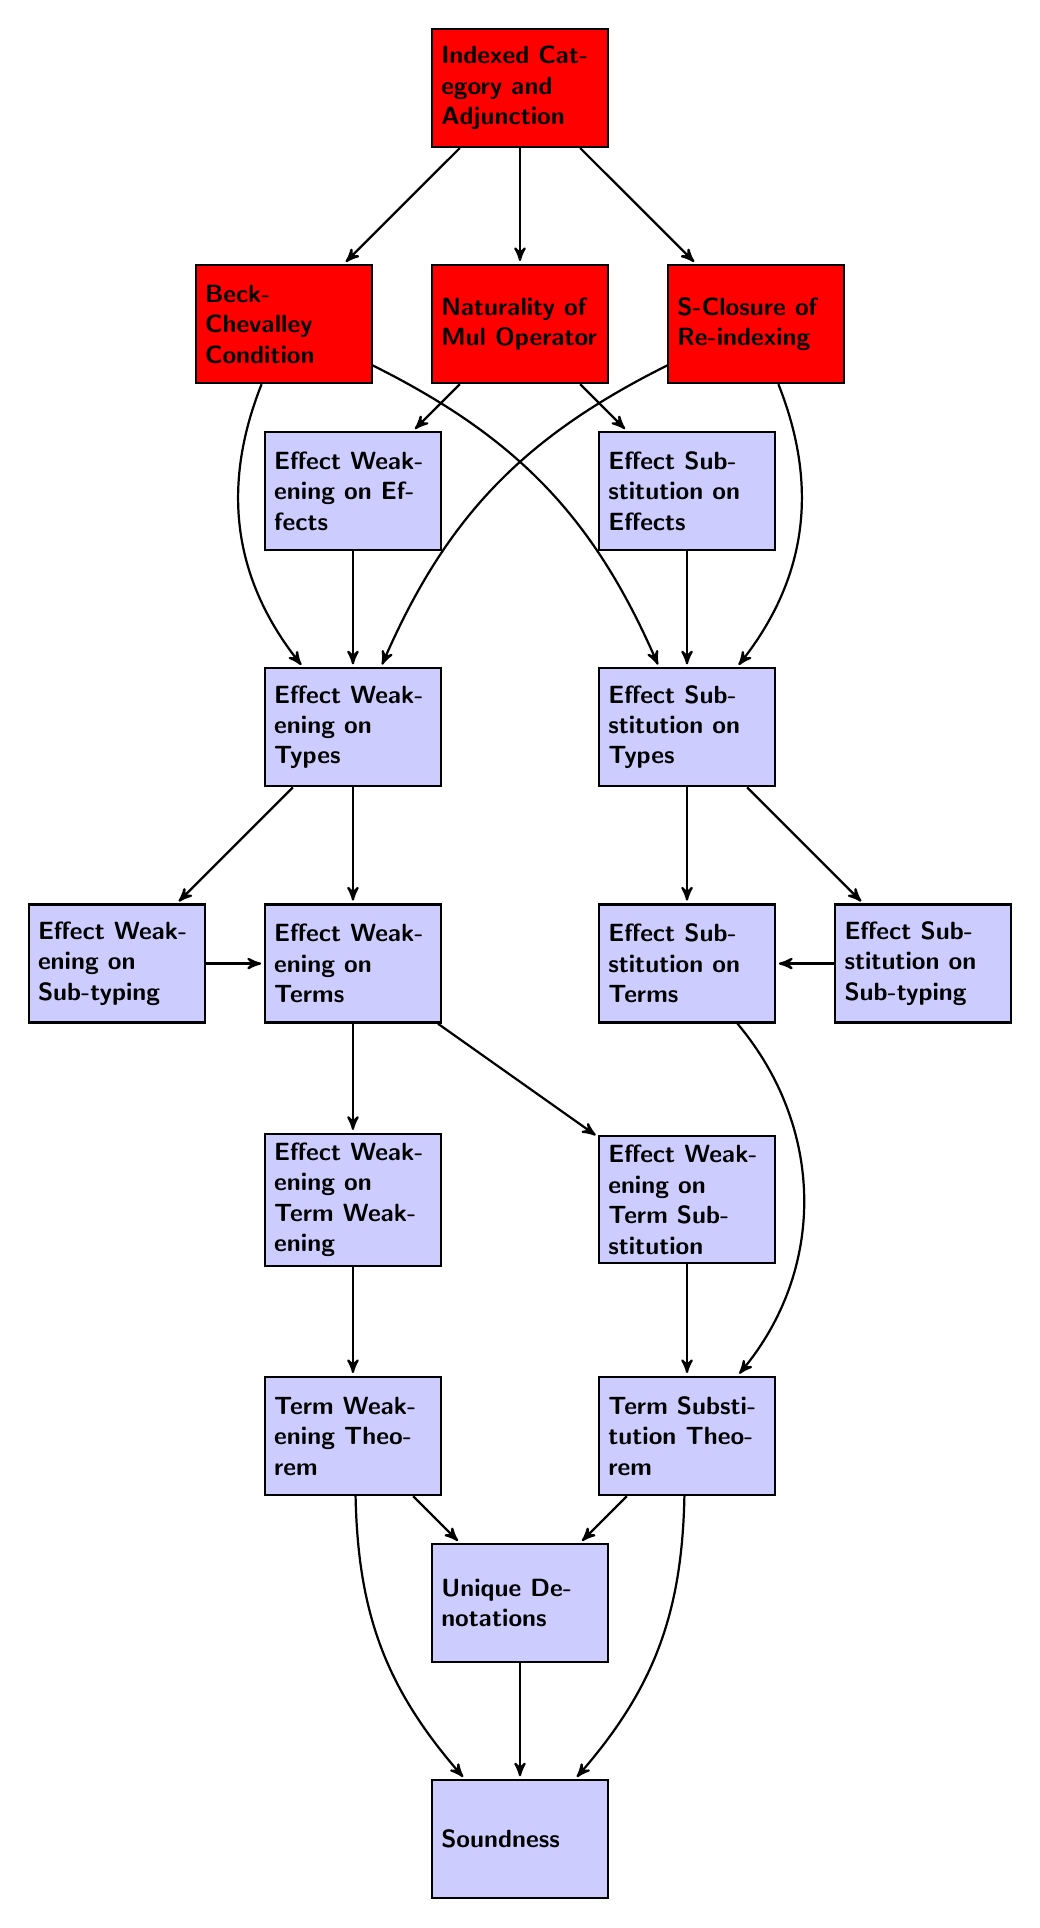
\begin{tikzpicture}[->,>=stealth',shorten >=1pt,auto,node distance=3cm,
    thick,main node/.style={rectangle,fill=blue!20,draw,
    font=\sffamily\small\bfseries,minimum size=15mm}]

    \node[main node,text width=20mm, fill=red] (IndexCategory) {Indexed Category and Adjunction};
    \node[main node,text width=20mm, fill=red] (MulNaturality) [below of=IndexCategory] {Naturality of Mul Operator};

    \node[main node,text width=20mm, fill=red] (BeckChevalley) [left of=MulNaturality]{Beck-Chevalley Condition};
    \node[main node,text width=20mm, fill=red](SClosure) [right of=MulNaturality]{S-Closure of Re-indexing};

    \node[main node, text width=20mm](EffectWeakeningEffects) [below left of=MulNaturality]{Effect Weakening on Effects};

    \node[main node, text width=20mm](EffectSubEffects) [below right of=MulNaturality]{Effect Substitution on Effects};

    \node[main node, text width=20mm](EffectWeakeningTypes)[below of=EffectWeakeningEffects]{Effect Weakening on Types};

    \node[main node, text width=20mm](EffectSubTypes)[below of=EffectSubEffects]{Effect Substitution on Types};

    \node[main node, text width=20mm](EffectWeakeningTerms)[below of=EffectWeakeningTypes]{Effect Weakening on Terms};

    \node[main node, text width=20mm](EffectSubTerms)[below of=EffectSubTypes]{Effect Substitution on Terms};

    \node[main node, text width=20mm](EffectWeakeningSubtyping)[left of=EffectWeakeningTerms]{Effect Weakening on Sub-typing};

    \node[main node, text width=20mm](EffectSubSubtyping)[right of=EffectSubTerms]{Effect Substitution on Sub-typing};

    \node[main node, text width=20mm](EffectWeakeningWeakening)[below of=EffectWeakeningTerms]{Effect Weakening on Term Weakening};

    \node[main node, text width=20mm](EffectWeakeningSubstitution)[below of=EffectSubTerms]{Effect Weakening on Term Substitution};

    \node[main node, text width=20mm](TermWeakening)[below of=EffectWeakeningWeakening]{Term Weakening Theorem};

    \node[main node, text width=20mm](TermSubstitution)[below of=EffectWeakeningSubstitution]{Term Substitution Theorem};

    \node[main node, text width=20mm](UniqueDenotations)[below left of=TermSubstitution]{Unique Denotations};

    \node[main node, text width=20mm](Soundness)[below of=UniqueDenotations]{Soundness};

    \draw [->] (IndexCategory) edge (BeckChevalley) (IndexCategory) edge (MulNaturality) (IndexCategory) edge (SClosure);
    \draw [->] (MulNaturality) edge (EffectWeakeningEffects) (MulNaturality) edge (EffectSubEffects);

    
    \draw [->] (EffectWeakeningEffects) edge (EffectWeakeningTypes) (EffectSubEffects) edge (EffectSubTypes);

    \draw [->] (EffectWeakeningTypes) edge (EffectWeakeningSubtyping) (EffectSubTypes) edge (EffectSubSubtyping);

    
    \draw [->] (EffectWeakeningSubtyping) edge (EffectWeakeningTerms) (EffectSubSubtyping) edge (EffectSubTerms);


    \draw [->] (EffectWeakeningTypes) edge (EffectWeakeningTerms) (EffectSubTypes) edge (EffectSubTerms);

    \draw [->] (EffectWeakeningTerms) edge (EffectWeakeningSubstitution) (EffectWeakeningTerms) edge (EffectWeakeningWeakening);

    \draw [->] (EffectWeakeningWeakening) edge (TermWeakening) (EffectWeakeningSubstitution) edge (TermSubstitution);

    \draw [->] (EffectSubTerms) edge [bend left=40] (TermSubstitution);
    \draw [->] 
        (BeckChevalley) edge [bend right=30] (EffectWeakeningTypes)
        (SClosure) edge [bend right=20] (EffectWeakeningTypes)
        (BeckChevalley) edge [bend left=20]  (EffectSubTypes)
        (SClosure) edge [bend left=30] (EffectSubTypes);
    

    \draw [->] (TermWeakening) edge (UniqueDenotations) (TermSubstitution) edge (UniqueDenotations) (TermWeakening) edge [bend right=20] (Soundness)
    (TermSubstitution) edge [bend left=20] (Soundness)
    (UniqueDenotations) edge (Soundness);
  \end{tikzpicture}
\caption{A road map of the proof dependencies. Assumptions in red, theorems in blue}
\end{figure}


\section{Denotations}
We are now equipped to define the denotations of structures in the language. Firstly, we shall define the denotation of the well-formed-ness relation on effects. As stated earlier, the denotation of an effect is a morphism $\deno{\typerelation{\P}{\e}{\effect}}$ in $\C$.

\[
    \deno{\typerelation{\P}{e}{\effect}} = \deno{\e} \after \term{I}: \rightarrow U
    \quad\quad
    \deno{\typerelation{\P,\a}{\a}{\effect}} = \pp: I\times U \rightarrow U
\]\[
    \deno{\typerelation{\P, \b}{\a}{\effect}} = \deno{\typerelation{\P}{\a}{\effect}}\after\p: I\times U\rightarrow U
\]\[
    \deno{\typerelation{\P}{\e_1\dot \e_2}{\effect}} = \Mul(\deno{\typerelation{\P}{\e_2}{\effect}},\deno{\typerelation{\P}{\e_1}{\effect}}): I \rightarrow U
\]

Using these denotations, we are now equipped to define the denotations of types. As stated above, types that are well formed in $\P$ are denoted by objects in the fibre category $\C(I)$ given by the denotation of $\P$. (\todo{Have I explained that $\deno{\P} = I$?}) 

Since the fibre category $\C(I)$ is S-Closed, it has objects for all ground types, a terminal object, graded monad $\T{}{}$, exponentials, products, and co-product over $\1+\1$.

\[
    \deno{\typerelation{\P}{\U}{\type}} = \1
    \quad\quad
    \deno{\typerelation{\P}{\B}{\type}} = \1+\1
    \quad\quad
    \deno{\typerelation{\P}{\g}{\type}} = \deno{\g}
\] 

\[
    \deno{\typerelation{\P}{\ab}{\type}} = (\deno{\typerelation{\P}{B}{\type}})^{(\deno{\typerelation{\P}{A}{\type}})}
\]

\[
    \deno{\typerelation{\P}{\mea}{\type}} =\T{\deno{\typerelation{\P}{\e}{\effect}}}{\deno{\typerelation{\P}{A}{\type}}}
    \quad\quad
    \deno{\typerelation{\P}{\all{\a}{A}}{\type}} =\allI(\deno{\typerelation{\P,\a}{A}{\type}})
\]


By using the terminal objects and products present in each fibre, we can now derive denotations of type-environments. $\deno{\oke{\P}{\G}}$ should be an object in the fibre induced by $\P$, $\C(I)$.

\[
    \deno{\wellformedok{\P}{\nil}} = \1
    \quad\quad
    \deno{\wellformedok{\P}{\gax}} = (\deno{\wellformedok{\P}{\G}} \times \deno{\typerelation{\P}{A}{\type}})
\]

\todo{Introduce the subtyping relation up above.}
Another construction that is important is the denotation of sub-typing. For each instance of the subtyping relation in $\P$, $A\subtypep B$, there exists a denotation in the fibre induced by $\P$. $\deno{A\subtypep B} \in\C(I)(A, B)$. Since the fibres are S-closed, the ground-instances of the sub-typing relation exist in each fibre anyway.


\[
    \deno{\g_1\subtypep \g_2} = \deno{\g_1\subtypeg \g_2}
    \quad
    \deno{\ab \subtypep \fntype{A'}{B'}} = \deno{B\subtypep B'}^{A'}\after B^{\deno{A'\subtypep A}}
\]

\[
    \deno{\M{\e_1}{A}\subtypep\M{\e_2}{B}} = \deno{\e_1\subeffectp\e_2}\after\T{\e_1}{\deno{A\subtypep B}}
    \quad    
    \deno{\all{\a}{A}\subtypep\all{\a}{B}} = \allI{\deno{A\subtypepa B}}
\]

This finally gives us the ability to express the denotations of well-typed terms in an effect environment, $\P$ as morphisms in the fibre induced by $\P$, $\C(I)$.  Writing $\G_I$ and $A_I$ for $\deno{\wellformedok{\P}{\G}}$ and $\deno{\typerelation{\P}{A}{\type}}$, we can derive $\deno{\gpetyperelation{v}{A}}$ as a morphism in $\C(I)(\G_I, A_I)$.

Since each fibre is an S-category, for each ground constant, $\const{A}$, there exists $c: \1 \rightarrow A_I$ in $\C(I)$.

\todo{Make these more readable/fix spacing}
\[
    \treerule{Unit}{\wellformedok{\P}{\G}}{\deno{\etyperelation{\P}{\G}{\u}{\U}} = \term{\G} : \G_I \rightarrow \1}
    \quad
    \treerule{Const}{\wellformedok{\P}{\G}}{\deno{\etyperelation{\P}{\G}{\const{A}}{A}} = \deno{\const{A}} \after \term{\G} : \G \rightarrow \deno{A}}
\]

\[
    \treerule{True}{\wellformedok{\P}{\G}}{\deno{\etyperelation{\P}{\G}{\t}{\B}} = \inl \after \term{\G} : \G \rightarrow \deno{\B} = \1+\1}
    \quad
    \treerule{False}{\wellformedok{\P}{\G}}{\deno{\etyperelation{\P}{\G}{\f}{\B}} = \inr \after \term{\G} : \G \rightarrow \deno{\B} = \1+\1}
\]

\[
    \treerule{Var}{\wellformedok{\P}{\G}}{\deno{\etyperelation{\P}{\gax}{x}{A}} = \pp: \G \times A \rightarrow A}
    \quad    
    \treerule{Weaken}{f = \deno{\gpetyperelation{x}{A}}: \G \rightarrow A}{\deno{\etyperelation{\P}{\gby}{x}{A}} = f \after \p: \G \times B \rightarrow A}
\]

\[
    \treerule{Lambda}{f = \deno{\etyperelation{\P}{\gax}{v}{B}} : \G \times A \rightarrow B}{\deno{\etyperelation{\P}{\G}{\lam{x}{A}{v}}{\ab}} = \cur{f} : \G \rightarrow (B)^A}
\]

\[
    \treerule{Subtype}{f = \deno{\etyperelation{\P}{\G}{v}{A}} : \G \rightarrow A\s\s g = \deno{A \subtypep B}}{\deno{\etyperelation{\P}{\G}{v}{B}} = g \after f : \G \rightarrow B}
    \quad 
    \treerule{Return}{f = \deno{\etyperelation{\P}{\G}{v}{A}}}{\deno{\etyperelation{\P}{\G}{\return{v}}{\moa}} = \point{A} \after f}   
\]

\[
    \treerule{If}{f = \deno{\etyperelation{\P}{\G}{v}{\B}}: \G\rightarrow\1+\1 \s\s g = \deno{\etyperelation{\P}{\G}{v_1}{\mea}}\s\s h = \deno{\etyperelation{\P}{\G}{v_2}{\mea}}}{\deno{{\etyperelation{\P}{\G}{\ifthenelse{\e}{A}{v}{v_1}{v_2}}{\mea}}} = \app\after((\fld{\cur{g\after\pp}}{\cur{h\after\pp}}\after f)\times \idg)\after \diag{\G} : \G \rightarrow \tea}    
\]

\[
    \treerule{Bind}{f = \deno{\etyperelation{\P}{\G}{v_1}{\M{\e_1}{A}} : \G \rightarrow \T{\e_1}{A}\s\s g = \deno{\etyperelation{\P}{\gax}{v_2}{\M{\e_2}{B}}}}: \G \times A \rightarrow \T{\e_2}{B}}{\deno{\etyperelation{\P}{\G}{\doin{x}{v_1}{v_2}}{\M{\e_1 \dot \e_2}{B}}} = \bind{\e_1}{\e_2}{B} \after \T{\e_1}{g} \after \tstrength{\G}{A}{\e_1} \after \pr{\idg}{f}: \G \rightarrow \T{\e_1 \dot \e_2}{B}}  
\]

\[
    \treerule{Apply}{f = \deno{\gpetyperelation{v_1}{\ab}}: \G \rightarrow (B)^{A} \s\s g=\deno{\gpetyperelation{v_2}{A}}: \G \rightarrow A}{\deno{\gpetyperelation{\apply{v_1}{v_2}}{\b}}= \app\after\pr{f}{g}: \G \rightarrow B }
\]

\[
    \treerule{Effect-Lambda}{f = \deno{\etyperelation{\P,\a}{\G}{v}{A}}: \ciuw(\G, A)}{\deno{\gpetyperelation{\elam{\a}{A}}{\all{\e}{A}}} = \bar{f}: \C(I)(\G, \allI(A))}    
    \quad
    \treerule{Effect-App}{g=\deno{\gpetyperelation{v}{\all{\a}{A}}}: \C(I)(\G, \allI(A))\s\s h = \deno{\typerelation{\P}{\e}{\effect}}: \ciu}{\deno{\gpetyperelation{\eapp{v}{\e}}{A\ssub{\a}{\e}}} = \pr{\Id{I}}{h}\star(\e_{\deno{\typerelation{\P,\b}{A\ssub{\a}{\b}}{\type}}})\after g: \C(I)(\G, A\ssub{\a}{\e})}
\]


\section{Substitution and Weakening Theorems}



\end{document}